\subsection{Full-model implementation and frequency preservation}
\label{sec:kam-control-experiment}
The feedback is integrated on all $64$ modes for $12$ s, using the
two-mode COMSOL integral fit certified in
Section~\ref{sec:validated-integral-learning}. The initial low state is
the phase-zero Fourier candidate and all higher modal positions and
velocities are zero. A separate high-accuracy integration of the
four-dimensional learned Hamiltonian supplies an implementation
reference. The plant is actuated through the physical tip force and moment.
The maximum canonical state difference is $1.54\times10^{-10}$,
the relative learned-energy change is below $2.64\times10^{-9}$,
and the full physical work-balance residual is below
$6.06\times10^{-17}$ J. The sampled field and gradient peaks are
$0.890325$ mT and $0.0256844$ T/m. Figure~\ref{fig:kam-magnetic-control}
compares this trajectory with the same initial state under passive
damping, for which the learned energy decreases by $99.8726\%$.
The numerical trajectory is an implementation check; the all-time
envelopes come from the preceding interval proof.
An independent implementation integrates the low Hamiltonian separately
and propagates each of the $62$ high damped oscillators by its exact
exponential response to piecewise-linear force demands. Force-grid
steps of $1$, $0.5$ and $0.25$ ms give maximum tip differences from the
full-state integration of $1.073$, $0.277$ and $0.106$ nm, respectively.
Every high-mode homogeneous transient is retained. This check separates
time-step error from modal truncation and supports the full-state
implementation. The resulting differences measure numerical convergence;
the rigorous bounds are supplied by the interval proof.

\paragraph{Independent online COMSOL feedback.}
The complete nodal beam is also solved with the CHNN feedback inside
COMSOL. The first two modal coordinates and velocities are projected
from its current beam state; two global algebraic equations enforce
the learned Legendre inverse. The physical tip force and magnetic
moment are recomputed online. This experiment is distinct from the
prescribed-field S-path replay.
Generalized-alpha integration uses $\rho_\infty=0$, a nonlinear relative
tolerance of $10^{-8}$ and fixed steps. Table~\ref{tab:comsol-kam-refinement}
reports four $4$ s refinements and compares them at common sampled
times with the independent full-state Python run.
At the finest step, the maximum relative change in the learned energy
is $0.0002958$. These numerical
errors are reported separately from the analytic KAM and all-time
amplitude certificates. Adaptive stepping stalled at very small steps
in two preliminary runs; fixed stepping completed each refinement.

\begin{table}[t]
\centering\small
\caption{Online COMSOL feedback versus independent Python
integration. Errors are in $\mu$m; no step-size tolerance is interpreted
as a rigorous error bound.}
\label{tab:comsol-kam-refinement}
\begin{tabular}{rrr}
\toprule
Step (ms) & Tip RMSE & Maximum tip difference\\
\midrule
1 & 147.852 & 355.845\\
0.5 & 41.356 & 99.176\\
0.25 & 12.006 & 28.161\\
0.125 & 3.848 & 8.658\\
\bottomrule
\end{tabular}
\end{table}

The two certified physical angular frequencies are approximately
$11.41719351$ and $70.24034116$ rad/s. Their exact specification and
all-integer Diophantine bound follow from the KAM certificate under
the stated time normalization. Magnetic feedback
therefore preserves a certified nonresonant frequency pair while
compensating damping. The complete nonlinear command contains the
harmonics determined by the torus; it is not approximated by two
sinusoidal inputs when invoking the lifting theorem. The rigorous
state and command envelopes provide a simultaneous amplitude check.
The operating-domain fraction is examined separately in
Section~\ref{sec:measure-numerical}.

\begin{figure*}[t]
\centering
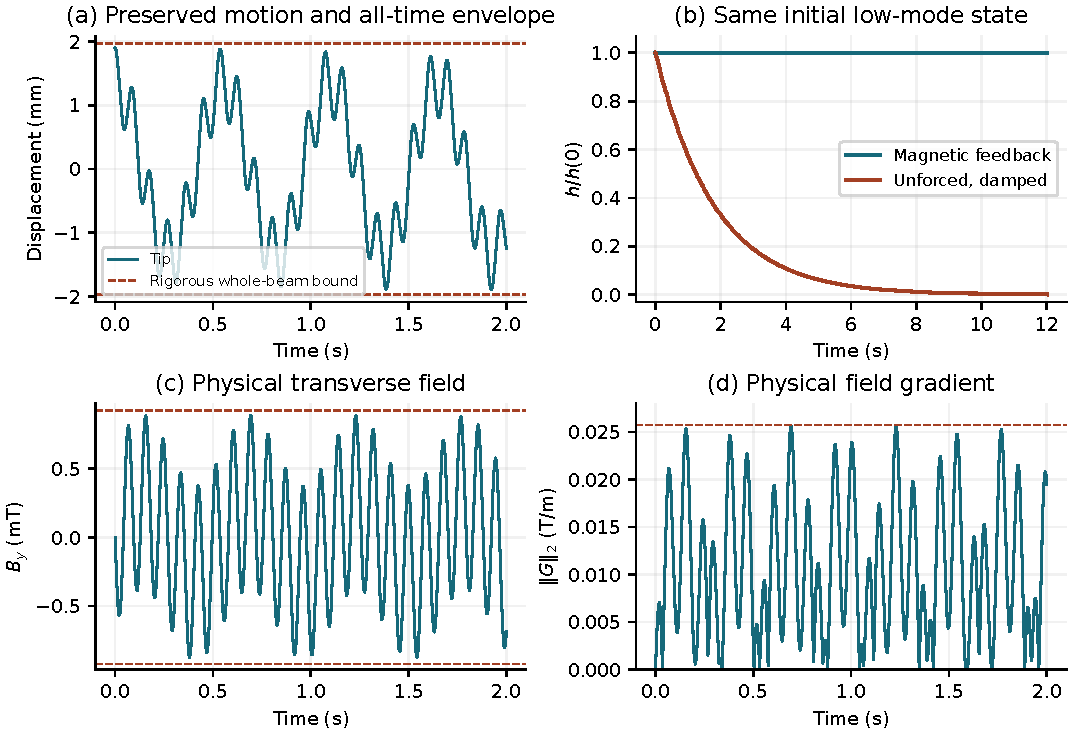
\includegraphics[width=\textwidth]{figures/fig_kam_magnetic_control.pdf}
\caption{Magnetic preservation of the COMSOL-integral learned
Hamiltonian on the complete exported modal FE plant. The higher modes
start at zero and undergo a decaying transient toward their unique
quasiperiodic response graph. Dashed bounds in (a), (c) and (d) are
validated all-phase bounds, including that startup. The field and
gradient in (c,d) jointly realize physical tip force and torque.
Panels (a,c,d) show the first $2$ s; panel (b) shows the complete $12$ s run.}
\label{fig:kam-magnetic-control}
\end{figure*}
